 \chapter{Экономический раздел}

 \section{Введение}

 Целью дипломной работы является доработка системы дистанционного обучения МАИ с целью адаптации системы на основе поступающей информа\-ции о времени, которое студент затрачивает для ответов на задачи в процессе тестирования. На основании анализа времени ответа делается вывод о том, не было ли у студента заранее приготовленных ответов не задачи теста.
В основной части диплома описывается математическое обеспечение системы и программная реализация, которые представляют собой завершенный прог\-раммный продукт, готовый для продажи на рынке программного обеспечения.
В экономической части диплома производится расчёт затрат, которые несёт разработчик программного обеспечения системы дистанционного обучения МАИ. Исходя из затрат формируется стоимость проекта в целом. По результа\-там оценки стоимости проекта производится расчёт экономической эффектив\-ности.

\section{Сетевой график}

Сетевой график представляет собой графическое отображение этапов ра\-бот, которые необходимо провести для завершения дипломного проекта. С помощью сетевого графика можно рассчитать спрогнозировать общее время, которое потребуется для выпол\-нения проекта, а так же вычислить вероят\-ность выпол\-нения проекта в срок.

\subsection{Таблица этапов работ}
По каждому этапу дипломной работы указано минимальное время выпол\-нения этапа и максимальное время выпол\-нения этапа. Исходя из этих зна\-чений рассчитывается ожидаемое время ответа:
$$
t_{exp} = \frac{2t_{min}+3t_{max}}{5}
$$

Дисперсия времени работы вычисляется по формуле
$$
t_{exp} = \left( \frac{t_{max} - t_{min}}{5} \right)^2
$$

По результатам расчётов построим таблицу
\begin{myTable}
\hline
Этап & Событие             & Шифр & Работа                                        & $t_{min}$ & $t_{max}$ & $t_{exp}$ & $\sigma$\\
\hline
1    & Изучение литературы & 1-4  & Изучение литературы по основной части диплома & 2         & 5         &  3,8      &  0,36    \\
\cline{3-8}
&

&
1-12&
Изучение литературы по экономической части&
3&
6&
4,8&
0,36
\\
\cline{3-8}
&

&
1-10&
Изучение литературы по охране труда и окружающей среды&
1&
4&
2,8&
0,36
\\
\hline
2&
Окончание доработки СДО&
2-7&
Анализ структуры и программного кода СДО&
6&
9&
7,8&
0,36
\\
\hline
3&
Получен список необходимых доработок&
3-2&
Доработка СДО для получения экспериментальных данных и оценки параметров модели&
4&
8&
6,4&
0,64
\\
\hline
4&
Необходимость построения математической модели&
4-5&
Изучение математических методов моделирования времени ответа в СДО&
2&
5&
3,8&
0,36
\\
\hline
5&
Завершение математической модели&
5-6&
Применение математической модели для анализа времени ответа&
7&
11&
9,4&
0,64
\\
\cline{3-8}
&

&
5-2&
Описание математической модели&
6&
9&
7,8&
0,36
\\
\hline
7&
Оценка параметров модели&
7-8&
Оценка по экспериментальным данным параметров модели &
7&
10&
8,8&
0,36
\\
\cline{3-8}
&

&
7-9&
Применение модели к реальным входным данным&
2&
5&
3,8&
0,36
\\
\hline
8&
Прогнозирование ответа на основании модели&
8-9&
Получение результатов обработки реальных данных&
3&
6&
4,8&
0,36
\\
\hline
9&
Построение таблиц, диаграмм, анализ полученных данных&
9-14&
Оформление результатов практической части&
4&
7&
5,8&
0,36
\\
\hline
10&
Раздел "Охрана труда и окружающей среды"&
10-11&
Написание теоретического материала раздела "Охрана труда и окружающей среды"&
3&
5&
4,2&
0,16
\\
\hline
11&
Расчет кондиционирования&
11-14&
Проведение расчётов&
6&
8&
7,2&
0,16
\\
\hline
12&
Раздел "Экономическая эффективность"&
12-13&
Написание теоретического материала раздела "Экономическая эффективность"&
2&
5&
3,8&
0,36
\\
\hline
13&
Построение сетевого графика&
13-14&
Проведение расчётов&
6&
9&
7,8&
0,36
\\
\hline
14&
Оформление готового диплома&
-
&
Оформление полученных результатов&
&

&

&
\\
\hline
\end{myTable}

\subsection{Построение сетевой модели}

Построим на основании таблицы из п. (1.2.1) «Таблица этапов работ» сетевой график. Круги обозначают события, стрелками обозначены работы. Подписи над стрелками указывают ожидаемое время выполнения работы.
\\
\begin{figure}[ht!]
\centering 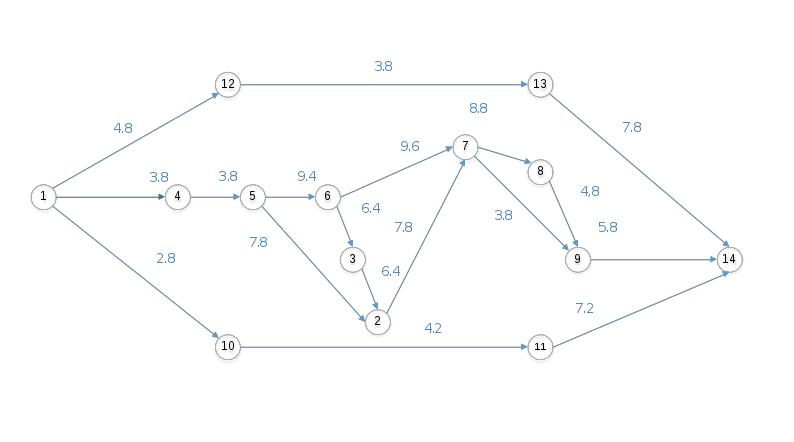
\includegraphics[bb=0 0 437 243]{Setevoy_Grafik.jpg}
\caption{Сетевой график}
\end{figure}
\\
\subsection{Анализ сетевой модели.}

Путём в сетевой модели называется последовательность работ, соединя\-ющая две любые работы на графике (если такая последовательность сущест\-вует)
Введём обозначения: $L_{1(i)}$ - путь, предшествующий событию $i$, $L_{2(i)}$ - путь, следующий за событием $i$.

Критический путь на сетевой модели (последовательность событий от начала проекта к концу проекта, имеющая максимальную длину):
$$
L = 1-4-5-6-3-2-7-8-9-14
$$

Длина пути $T(L) = \sum\limits_{i-j}t_{i-j}$ (где $t_{i-j}$ - длительность работы с меткой $i-j$) - сумма длительностей работ, которые выполняются при следовании по пути. Длина критического пути:
$$
T_{\mbox{кр}}(L) = 3.8+3.8+9.4+6.4+6.4+7.8+8.8+4.8+5.8 = 50.6
$$
Ранний срок наступления события: $t_{\mbox{р}(i)} = max(T(L_{1(i)}))$\\
Ранний срок начала работы: $t_{\mbox{рн}(i-j)} = max(T(L_{1(i)}))$\\
Ранний срок окончания работы: $t_{\mbox{ро}(i-j)}= t_{\mbox{р}(i)} - t_{(i-j)} = max(T(L_{1(i)})) + t_{(i-j)} $\\
Поздний срок наступления события: $t_{\mbox{п}(i)}= T_{\mbox{кр}}(L) -  max(T(L_{2(i)}))$\\
Поздний срок начала работы: $t_{\mbox{пн}(i-j)}= t_{\mbox{по}(i)} - t_{(i-j)}$\\
Поздний срок окончания работы: $t_{\mbox{по}(i-j)} = t_{\mbox{п}(j)}= T_{\mbox{кр}}(L) -  max(T(L_{2(i)}))$\\
Общий резерв времени работы: $R_{(i-j)} = t_{\mbox{по}(i-j)} - t_{\mbox{ро}(i-j)} =  t_{\mbox{п}(j)} -  t_{\mbox{р}(j)} -  t_{(i-j)}$\\
Свободный резерв времени работы: $r_{(i-j)} = t_{\mbox{р}(i-j)} - t_{\mbox{ро}(i-j)} =  t_{\mbox{р}(j)} -  t_{\mbox{р}(i)} -  t_{(i-j)}$\\
Резерв времени события: : $r_{(i)} = t_{\mbox{п}(i)} - t_{\mbox{р}(i)} $

Результат расчёта параметров для сетевой модели работы над дипломным проектом представлен в таблице (утолщённым шрифтом обозначены работы, принадлежащие критическому пути):
\begin{myTableSecond}
\hline
Шифр & $t_{exp}$ & $\sigma$ &  $t_{\mbox{рн}(i-j)}$ $t_{\mbox{р}(i)}$ & $t_{\mbox{ро}(i-j)}$ & $t_{\mbox{пн}(i-j)}$ & $t_{\mbox{по}(i-j)}$ $t_{\mbox{п}(j)}$ & $R_{(i-j)}$ & $r_{(i-j)}$ & $r_{(i)}$\\
\hline
1-4&
3,8&
0,36&
0&
3,8&
8,8&
12,6&
8,8&
0&
8,81\\
\hline
1-12&
4,8&
0,36&
0&
4,8&
49,4&
54,2&
49,4&
0&
49,4\\
\hline
1-10&
2,8&
0,36&
0&
2,8&
51,6&
54,4&
51,6&
1,4&
51,6\\
\hline
2-7&
7,8&
0,36&
29,8&
37,6&
38,6&
46,4&
8,8&
0&
8,8\\
\hline
3-2&
6,4&
0,64&
23,4&
23,4&
32,2&
38,6&
15,2&
6,4&
15,2\\
\hline
4-5&
3,8&
0,36&
3,8&
7,6&
12,6&
16,4&
8,8&
2,7&
8,8\\
\hline
5-6&
9,4&
0,64&
7,6&
17&
16,4&
25,8&
8,8&
9,6&
8,8\\
\hline
5-2&
7,8&
0,36&
15,4&
15,4&
30,8&
38,6&
23,2&
14,4&
23,2\\
\hline
6-3&
6,4&
0,64&
17&
23,4&
25,8&
32,2&
8,8&
0&
8,8\\
\hline
6-7&
9,6&
0,04&
26,6&
26,6&
36,8&
46,4&
19,8&
11&
19,8\\
\hline
7-8&
8,8&
0,36&
37,6&
46,4&
46,4&
55,2&
8,8&
0&
8,8\\
\hline
7-9&
3,8&
0,36&
37,6&
51,2&
56,2&
60&
8,8&
0&
8,8\\
\hline
8-9&
4,8&
0,36&
46,4&
51,2&
55,2&
60&
8,8&
0&
8,8\\
\hline
9-14&
5,8&
0,36&
51,2&
57&
60&
65,8&
8,8&
0&
8,8\\
\hline
10-11&
4,2&
0,16&
2,8&
7&
54,4&
58,6&
51,6&
0,2&
51,6\\
\hline
11-14&
7,2&
0,16&
7&
14,2&
58,6&
65,8&
51,6&
0&
51,6\\
\hline
12-13&
3,8&
0,36&
4,8&
8,6&
54,2&
58&
49,4&
0&
49,4\\
\hline
13-14&
7,8&
0,36&
8,6&
16,4&
58&
65,8&
49,4&
0&
49,4\\
\hline
\end{myTableSecond}

Директивный срок выполнения проекта составляет 122 дня, при этом длина критического пути 50.6 дней – таким образом, проект будет завершён в строк и нет необходимости перестраивать сетевой график проекта. Сумма дисперсий работ, лежащих на критическом пути, составляет 4.08. Среднеквад\-ратическое отклонение для критического пути составляет $\sqrt{4.08} = 2.02$ . Доверительный интервал для срока выполнения всех работ имеет вид $[50.6-2.02,50.6+2.02 ] \sim [30.58, 52.62]$. Вероятность выполнения работы в срок составляет $P=\Phi((122-50.6)/2.02)=\Phi(35.3)\sim 1$, где $\Phi(x)$ – функция Лапласа.

\section{Расчет затрат}

В разделе описаны основные затраты разработчика, влияющие на цену конечного продукта: расходные материалы, аренда помещений, заработная плата и т.д.

\subsection{Приобретение материалов}

Для проведения процесса разработки программного обеспечения необхо\-димо приобрести оборудование для разработчика (ноутбук) и пакет прик\-ладных программ для разработчика.

\subsubsection{Оборудование}
Для выбора оборудования произведём сравнительный анализ нескольких моделей с использованием сервиса Яндекс.Маркет (http://market.yandex.ru/).
Сравнение произведём между тремя моделями стоимостью до 22 000 руб. от производителей “Lenovo”, “Dell” “Samsung”.

\begin{table}[H]
\begin{center}
\begin{tabular}{|p{3.5cm}|p{3.6cm}|p{3.6cm}|p{3.4cm}|}
\hline
Характеристика & \multicolumn{3}{|c|}{Модель}\\
\hline
Название&
Lenovo THINKPAD L420&
DELL Vostro 1440&
Samsung 535U4C\\
\hline
Операционная система&
Win 7 Professional&
Win 7 Home Basic 64&
Win 7 Home Basic 64\\
\hline
Тип процессора&
Core i3&
Celeron&
Core i3\\
\hline
Частота процессора (МГц)&
2300&
2000&
1600\\
\hline
Размер оперативной памяти&
2&
2&
4\\
\hline
Тип экрана&
матовый&
матовый&
Глянец\\
\hline
Объём накопителя&
250&
320&
500\\
\hline
Время работы&
11&
8&
7\\
\hline
Графика&
интегрированная&
интегрированная&
дискретная\\
\hline
Вес&
2.24&
2.19&
1.81\\
\hline
Цена&
12 952&
13 855&
21 459\\
\hline
\end{tabular}
\end{center}
\end{table}

Т.к. работать с ноутбуком планируется не в одном и том же месте, а при постоянных перемещениях, то модель от Lenovo не подходит, т.к. обладает слишком большим весом. Так же Lenovo имеет самый маленький размер жесткого диска среди представленных моделей, а объём оперативной пяти у него не больше, чем у конкурентов.

Среди двух оставшихся моделей Samsung обладает более мощным гра\-фическим процессором (дискретным), большим объёмом жёсткого диска и малым весом, а так же большим объемом оперативной памяти. При этом Dell имеет более производительный процессор Intel, более долгое время работы от аккумулятора, а так же матовым экраном (это более эргономично для программиста) и меньшей ценой. Поэтому принимаем решение о покупке ноутбука DELL Vostro 1440 стоимостью N = 21459 руб. на основании сравни\-тельного анализа.

\subsubsection{Программное обеспечение}

Цикл разработки программного обеспечения включает в себя несколько этапов: анализ требований, проектирование системы, разработка програм\-много обеспечения. В таблице приведены затраты на минимально необходи\-мый список программного обеспечения по каждому этапу. Цены приведены в рублях, по курсу на 24.11.2013

\begin{table}[H]
\begin{center}
\begin{tabular}{|p{3.5cm}|p{3.6cm}|p{3.6cm}|p{3.4cm}|}
\hline
Название этапа&
Название ПО&
Цена ПО (руб.)\\
\hline
Анализ требований&
Trello&
1320\\
\hline
Проектирование системы&
Microsoft Visio&
19 499\\
\hline
Разработка ПО&
Sublime Text 3&
2310\\
\hline
\multicolumn{2}{|c|}{Итого} &23219\\
\hline
\end{tabular}
\end{center}
\end{table}

Итого, на приобретение программного обеспечения будет затрачено U = 23219 руб.

\subsection{Аренда помещений}

По причине того, что разработкой системы дистанционной системы обу\-чения занимается программист, который тратит на разработку не полный рабочий день, в качестве помещения для разработки будет использован ковор\-кинг-цетр недалеко от метро Шаболовская (т.к. это наиболее удобный для программиста район). Ссылка на сайт центра: http://www.matrixoffice.ru. Ком\-ната в коворкинг-центре включает всё, что нужно для работы: кресло, стол, высокоскоростной доступ в интернет.
В таблице произведён расчёт затрат на аренду помещения с учётом того, что цикл разработки займёт три месяца (сентябрь, октябрь, ноябрь)

\begin{table}[H]
\begin{center}
\begin{tabular}{|p{3.5cm}|p{3.6cm}|p{3.6cm}|}
\hline
Число рабочих дней на проект&
63\\
\hline
Количество рабочих часов в день&
4\\
\hline
Полное число часов&
252\\
\hline
Стоимость часа аренды&
200\\
\hline
Итого&
50400\\
\hline
\end{tabular}
\end{center}
\end{table}

Итого, затраты на аренду составят H = 50400 руб.

\subsection{Заработная плата}

При работе над экономической частью дипломного проекта необходимо рассчитать заработную плату сотрудникам, задействованным в работе над дипломом.

В работе над дипломным проектом принимают участие научный руко\-водитель, программист, консультанты. Для каждого специалиста вычисляется объём заработной платы, исходя из почасовой ставки и  времени, в течение которого специалист участвует  проекте

Расчёты приведены в таблице: Данные для вычисления почасовой зара\-ботной платы программиста получены с помощью сайта http://www.hh.ru/, данные по заработной плате научных руководителей и консультантов соот\-ветствуют зарплатам в Московском авиационном институте за 2013 г.
\begin{table}[H]
\begin{center}
\begin{tabular}{|p{3.5cm}|p{1.8cm}|p{1.6cm}|p{2.8cm}|p{2.1cm}|p{1.8cm}|}
\hline
Специалист&
Заработ\-ная плата&
Коли\-чество часов &
Количество часов на одного дипломника&
Почасовая оплата&
Заработ\-ная плата\\
\hline
Научный руководитель&
40000&
90&
24&
444&
10666\\
\hline
Консультант по экономической части&
40000&
90&
2&
444&
888\\
\hline
Консультант по охране труда и окружающей среды&
40000&
48&
2&
833&
1666\\
\hline
Программист&
-&
252&
-&
630&
158760\\
\hline
\multicolumn{5}{|c|}{Итого}&
171980\\
\hline
\end{tabular}
\end{center}
\end{table}

Итого затраты на заработную плату составят Z = 171980 руб.

\subsection{Транспортные расходы}

Затраты на транспорт фигурируют в работе над дипломным проектом, т.к. встречи между участниками проекта происходят на территории МАИ и каждый из работников затрачивает денежные средства на то, чтобы добраться до МАИ. Предполагается, что все участники добираются до на метро.

В таблице для каждого участника учтено количество поездок (опреде\-ляется исходя из этапов работы над дипломом), а так же полные затраты на транспорт за период написания диплома:
\begin{table}[H]
\begin{center}
\begin{tabular}{|p{3.5cm}|p{2.8cm}|p{2.6cm}|p{2.8cm}|}
\hline
Специалист&
Количество поездок&
Стоимость 1-ой поездки&
Итого\\
\hline
Научный руководитель&
16&
&
448\\
\cline{1-2}\cline{4-4}
Консультант по экономической части&
2&
&

56
\\
\cline{1-2}\cline{4-4}
Консультант по охране труда и окружающей среды&
2&
28
&
56
\\
\cline{1-2}\cline{4-4}
Программист&
20&
&
560\\
\hline
\multicolumn{3}{|c|}{Итого}&
1120\\
\hline
\end{tabular}
\end{center}
\end{table}

Итого расходы на транспорт составляют M = 1120 руб.

\subsection{Расходы амортизацию оборудования}

Оборудование, которое использовалось в ходе выполнения дипломной ра\-боты, подлежит амортизации. Амортизации подвергаются основные средства и нематериальные активы для переноса части их стоимости в цену производи\-мой продукции.

Согласно пункту 1.2.1.1 «Оборудование», основным оборудованием (сред\-ством производства) является ноутбук. Расчет амортизации произведём ли\-нейным способом:
$$
A = \frac{S\cdot n \cdot t}{ 100 \cdot T}
$$

В таблице приведены расшифровка и значения переменных в формуле.
\begin{table}[H]
\begin{center}
\begin{tabular}{|p{3.0cm}|p{3.8cm}|p{2.6cm}|}
\hline
Переменная&
Описание&
Значение\\
\hline
S&
Стоимость оборудования&
21459 руб.\\
\hline
n&
Годовая норма амортизации&
20 \%\\
\hline
t&
Время работы оборудования&
252 часа\\
\hline
T&
Эффективный срок работы оборудования&
1800 часов\\
\hline
\end{tabular}
\end{center}
\end{table}

Произведём расчёт согласно данным таблицы:
$$
A = \frac{21459\cdot 20 \cdot 252}{ 100 \cdot 1800} = 601 \mbox{ (руб.)}
$$

Таким образом, амортизация ноутбука за период написания диплома со\-ставит 601 руб.

\section{Социальные отчисления}

Работодателю необходимо произвести социальные отчисления с зарплаты работников в следующем размере:
Взносы в ФФОМС: 5.1\%\\
Взносы в ФСС: 2.9\%\\
Взносы в Пенсионный фонд: 22\%

Таким образом, на затраты на социальные отчисления составят (с учётом фонда оплаты труда из пункта 1.2.3 «Заработная плата»
$$
P = Z \cdot (5.1 + 2.9 + 22) = Z \cdot 30 = 171980 \cdot 30 = 51594 \mbox{ (руб.)}
$$

Итого, размер социальных выплат составит 51594 руб.

\subsection{Прочие расходы}

К прочим расходам относится мобильная связь. Исходя из того, что один комплект оператора «МТС», включающий 300 минут разговоров и неограни\-ченное количество смс стоит 500 руб. для каждого участника разработки диплома, то за 4 месяца для 4-х человек получаем
$$
B = 500 \cdot 4 \cdot 4 = 8000 \mbox{ (руб.)}
$$

Итого, общие расходы составляют 8000 руб.

\subsection{Накладные расходы}

К накладным расходам относятся затраты, не связанные прямо с разработ\-кой системы дистанционного обучения – например, приобретение литературы для разработчика. Накладные расходы принимаются в размере 5\% от фонда оплаты труда:
$$
D = FOT \cdot 5\% = 171980 \cdot 5 \% = 8599 \mbox{ (руб.)}
$$

Итого, накладные расходы составляют $8599 \mbox{ (руб.)}$

\section{Расчет экономической эффективности}

Для расчёта экономической эффективности нужно вычислить се\-бесто\-имость продукта, его цену продажи, а так же экономический эффект, который ожида\-ется от внедрения продукта

\subsection{Расчёт цены на продукт}

Чтобы рассчитать цену на продукт, необходимо вычис\-лить его себесто\-имость. Се\-бестоимость продукта с определяется как сумма всех затрат, вычис\-ленных в пункте 1.2 «Расчет затрат»:\\
\begin{math}
SS = D + B + P + A+M+H+U+N+Z = \\ 
=171980 + 8000 + 601 + 1120 + 50400 + 23219 + 21459 + 8599 + 51594 = 336972
\end{math}

Норма прибыли равна 5\%. НДС, который так же нужно учесть в цене, составляет 18\%. Тогда цена на продукт составит
$$
C = 336972 \cdot (100\% + 5\% + 18\%) = 414476 \mbox{ (руб.)}
$$

\section{Экономический эффект}

Экономический эффект, который принесёт внедрение доработок в систему дистанционного обучения, заключается в ликвидации недополученной при\-были за дополнительные занятия для студентов.

После внедрения системы появиться возможность выделить среди группы студентов, проходящих курсы в системе дистанционного обучения, тех обу\-чающихся, которые решают задачи теста с заранее имеющимися ответами.

Если студент использует  готовые ответы – он не до конца освоил нужный курс и нуждается в дополнительных занятиях. Оценим прибыль, которую институт может получить за один семестр по формуле:
$$
L = N \cdot i \cdot k \cdot V
$$

В таблице приведены расшифровка и значения переменных в формуле.
\begin{table}[H]
\begin{center}
\begin{tabular}{|p{3.0cm}|p{4.1cm}|p{2.6cm}|}
\hline
Переменная&
Описание&
Значение\\
\hline
N&
Количество студентов &
430\\
\hline
i&
Доля воспользовавшихся ответами&
15 \%\\
\hline
k&
Стоимость одного доп. занятия на курсах&
540 руб.\\
\hline
V&
Количество доп. занятий&
4 шт
\\
\hline
\end{tabular}
\end{center}
\end{table}

Таким образом, получаем:
$$
L = N \cdot i \cdot k \cdot V = 450 \cdot 15 \cdot 540 \cdot 4 =  139320 \mbox{ (руб.)}
$$

Итого, экономический эффект от системы дистанционного обучения сос\-тавит 139320 руб. в семестр.

\subsection{Экономическая эффективность}

Для расчёта экономической эффективности необходимо учесть расходы на внедрение системы и эксплуатацию сервиса.

Расходы на внедрение системы  вычисляются по формуле 
$$
C_{\mbox{вн}} = t_{\mbox{вн}}\cdot p,
$$
где $t_{\mbox{вн}} = 3$ часа - время, необходимое для установки системы на сервер и $p=630$ руб. - почасовая ставка программиста, который занимается развёр\-тыванием системы
$$
C_{\mbox{вн}} = 3 \cdot 630 = 1890 \mbox{ (руб.)},
$$

Расходы на эксплуатацию сервиса складываются из затрат на оплату сервера, который использует система дистанционного обучения:
$$
C_{\mbox{эксп}} = t_{\mbox{эксп}}\cdot c,
$$

где $t_{\mbox{эксп}} = 6$ мес. (расчёты производим за семестр) и  $c = 1200$ руб. – помесячная оплата сервера.
$$
C_{\mbox{эксп}} = 6 \cdot 1200 = 7200 \mbox{ (руб.)},
$$ 

Итого получаем срок окупаемости вложенных средств:
$$
T_{\mbox{ок}} = \frac{C_{\mbox{эксп}} + C_{\mbox{вн}} + C}{L} = \frac{7200+1890+414476}{139320} = 3.04 (\mbox{ семестра})
$$

Таким образом средства, вложенные в систему, будут возвращены в течение четырёх семестров.

\section{Вывод} 
В экономической части дипломной работы был произведён расчёт себес\-тоимости и цены продажи проекта.

Построен сетевой график выполнения дипломной работы. По графику найден критический путь и рассчитаны параметры сетевой модели для каждо\-го узла. По рассчитанным параметрам произведена оценка наиболее вероят\-ного срока выполнения проекта, а так же вычислена вероятность завершения проекта в срок.

Была проведена оценка затрат на введение и эксплуатацию системы, а так же оценка прибыли, которую принесёт проект. На основании этих данных определёна экономическая эффективность разработанной системы.

По результатам расчётов сделан вывод о том, что вложенные в систему средства будут возвращены инвестору в течение четырёх учебных семестров.